\documentclass[11pt,a4paper]{article}
\usepackage[margin=22mm]{geometry}
\usepackage[T1]{fontenc}
\usepackage{lmodern}
\usepackage{microtype}
\usepackage{setspace}
\usepackage{booktabs,tabularx,array}
\usepackage{enumitem}
\usepackage{xcolor}
\usepackage{tikz}
\usetikzlibrary{arrows.meta,positioning}
\usepackage[hidelinks]{hyperref}
\usepackage{fancyhdr}
\usepackage{titlesec}
\usepackage[section]{placeins}
\setstretch{1.04}
\setlength{\parindent}{0pt}
\setlength{\parskip}{5pt plus 1pt}
\setlist{nosep,leftmargin=1.5em}
\setlength{\emergencystretch}{2em}
\widowpenalty=10000
\clubpenalty=10000
\renewcommand{\arraystretch}{1.15}
\newcolumntype{Y}{>{\raggedright\arraybackslash}X}
\newcolumntype{P}[1]{>{\raggedright\arraybackslash}p{#1}}
\setcounter{tocdepth}{1}
\titleformat{\section}{\large\bfseries}{\thesection}{0.7em}{}
\titleformat{\subsection}{\normalsize\bfseries}{\thesubsection}{0.7em}{}
\titlespacing*{\section}{0pt}{12pt}{5pt}
\titlespacing*{\subsection}{0pt}{8pt}{3pt}
\pagestyle{fancy}
\fancyhf{}
\fancyhead[L]{\small CRAG continuous assessment report}
\fancyhead[R]{\small Draft 1}
\fancyfoot[C]{\thepage}
\setlength{\headheight}{14pt}
\newcommand{\blankfield}{\rule{0.49\textwidth}{0.35pt}}
% Draft metadata: complete only after author confirmation.
% Official registered title, project/module code, student number, supervisor
% and main evaluator deliberately remain blank.
% Author confirmed no personal contribution before May 2026.
% Future semester dates are provisional: January--May 2027.
% Source: supplied Downloads/main.tex; repository HEAD
% 35e2a0e7832654864076a2729cd434b6330dd136, inspected 29 October 2026.
% Inherited snapshot: 69727bb (4 April 2026), latest pre-May commit on HEAD ancestry.
% No May--July 2026 commits found on that ancestry; do not invent monthly activities.
% Survey figures cross-checked against local CSV aggregates; never attach raw identities.
% Source comments and author notes are drafting aids, not submission instructions.

% Opening layout adapted from Dethada/NUS-SoC-Report (David Zhu, 2024).
% See template-LICENSE.txt. Academic year remains unconfirmed.
\newcommand{\reportidentity}{%
{\large CP4101 Continuous Assessment Report\par}
\vfill
{\LARGE\bfseries CRAG: An Instructor-Governed, \\Course-Grounded RAG Platform for AI\\Teaching Assistants in Higher Education\par}
\vspace{3mm}
\vspace{2cm}
{\large By\par Ryan Chen Rui Yang\par}
\vfill
{\normalsize Department of Computer Science\par
School of Computing\par
National University of Singapore\par}
\vspace{1cm}
{\normalsize 2026/2027\par}}

\begin{document}
\hypersetup{pageanchor=false}
\newgeometry{left=3cm,right=3cm,top=3cm,bottom=3cm}
\begin{titlepage}
\centering
\reportidentity
\end{titlepage}
\begin{titlepage}
{\centering\reportidentity\par}
\vspace{1cm}
\begin{tabular}{@{}P{0.30\textwidth}P{0.63\textwidth}@{}}
Student number & A0272246E\\[6pt]
Project ID & H1352890\\[6pt]
Supervisor & Anand Bhojan\\[6pt]
Main Evaluator & Yap Hock Chuan, Roland\\[6pt]
Planned next semester & January--May 2027\\[6pt]
\end{tabular}
\end{titlepage}
\restoregeometry
\pagenumbering{roman}
\hypersetup{pageanchor=true}
\pagestyle{plain}

\section*{Abstract}
\addcontentsline{toc}{section}{Abstract}
This project develops CRAG, an instructor-governed, course-grounded AI tutoring platform, towards more dependable educational assistance and a defensible basis for studying student reasoning. It extends an existing student-built system rather than starting from a new chatbot. The inherited platform already connected course materials, student chat, instructor management, learning modes, quizzes and Discord. Work undertaken during May--October 2026 has focused on strengthening evidence handling, conversational support, instructor feedback, operational recovery and consent-aware research infrastructure.

The central problem is that a fluent, source-linked answer does not by itself establish factual support, appropriate instructional help or learning. CRAG therefore combines course-scoped retrieval with bounded corrective search, answer attribution review and explicit instructor approval. It also provides practice and follow-up activities through which students can explain, question and revise their understanding. The research direction uses Holistic Cognitive Development (HCD) to examine these processes while keeping operational activity distinct from validated educational outcomes.

Progress comprises an extended integrated platform, a baseline needs assessment reported in the IEEE TALE paper, and infrastructure for subsequent technical and educational evaluation. The next semester, provisionally January--May 2027, will prioritise reproducible answer-quality comparisons, source freshness and failure recovery, validated dialogue coding, and a feasible consented study of reasoning and revision. Historical prototype results and baseline preferences inform this work; they do not establish the effectiveness of the present implementation.

\clearpage
\begingroup
\small
\setlength{\parskip}{0pt}
\tableofcontents
\endgroup
\clearpage
\listoffigures
\addcontentsline{toc}{section}{\listfigurename}
\clearpage
\listoftables
\addcontentsline{toc}{section}{\listtablename}
\clearpage
\pagenumbering{arabic}
\pagestyle{fancy}

\section{Introduction}
\subsection{Problem and intended contribution}
Students need explanations that fit their course, remain traceable to teaching materials and help them work through uncertainty. General-purpose assistants provide flexible dialogue, but their answers can omit course assumptions or present plausible claims without adequate evidence. A course assistant also needs an accountable correction process: instructors must be able to identify a problematic answer, supply a reviewed response and communicate that update to the student.

CRAG addresses these needs as an integrated workflow. Instructors organise a course knowledge base and review answers; students ask questions, inspect sources and undertake practice; researchers examine eligible interactions with recorded context and provenance. The contribution lies in developing and investigating the relationships between these capabilities. Combining familiar components does not establish algorithmic novelty or educational superiority. The relevant questions concern whether the resulting system provides dependable support, workable instructor oversight and interpretable evidence about student reasoning.

The supplied IEEE TALE paper describes this platform and reports a CS3103 pre-use needs assessment alongside earlier prototype evidence~\cite{cragpaper}. This report extends that account with implementation progress through October 2026 and a proposed next-semester investigation.

\subsection{Objectives and completion criteria}
\begin{enumerate}[label=\textbf{O\arabic*.}]
\item \textbf{Improve course-grounded assistance.} Preserve course scope, retrieve evidence relevant to the question and expose supported citations. Evaluate correctness, requested-detail coverage, citation support and appropriate abstention separately.
\item \textbf{Make instructor governance effective.} Support answer review, correction, controlled reuse and student updates. Evaluate review effort, decision consistency and whether corrections reach the intended recipients.
\item \textbf{Support purposeful student interaction.} Connect Standard, Guided and Socratic modes with quizzes, follow-up discussion and revision tools. Investigate how students use these affordances rather than treating their availability as evidence of learning.
\item \textbf{Provide reliable operational and research foundations.} Preserve access control, recoverable workflows, ordered conversation records, consent eligibility and response provenance. Check these contracts through regression and synthetic integration tests.
\item \textbf{Develop and conduct a defensible evaluation.} Establish frozen technical comparisons and a feasible HCD-informed study, with independent judgements, participant accounting and explicit limits on causal interpretation.
\end{enumerate}

\subsection{Scope and research questions}
The implementation covers the FastAPI backend, student web application, instructor dashboard and optional Discord client, sharing Supabase data and external model services. Course material remains the default evidence source. Supplementary material may support chat while remaining outside quiz generation and selection.

Three questions guide the next phase. \textbf{RQ1:} How do corrective retrieval and answer review affect support, completeness, abstention, latency and cost relative to a fixed single-query RAG baseline? \textbf{RQ2:} How usable and effective is instructor review as a correction workflow? \textbf{RQ3:} What evidence of explanation, critique and justified revision appears in student interactions, and how does it relate to independently assessed understanding? These questions separate technical quality, workflow quality and educational outcomes.

\section{Literature review}
\subsection{Scope and organising argument}
This focused review examines retrieval and attribution, educational dialogue, instructor oversight and ethical learning analytics. It draws on primary research and the theoretical sources underlying the TALE paper, with additional work on corrective retrieval and contemporary educational assistants. It is a thematic review rather than an exhaustive systematic review: no complete database search or screening protocol is claimed. Its organising argument is that reliable educational assistance requires both inspectable evidence and opportunities for learners to exercise judgement.

\subsection{Retrieval improves access to knowledge but leaves support unresolved}
Lewis et al.\ combine parametric generation with retrieved non-parametric knowledge, demonstrating the value of retrieval for knowledge-intensive tasks~\cite{lewis}. This provides a foundation for using course materials as an explicit evidence collection. However, improvements on open-domain benchmarks do not determine whether a particular lecture passage supports a course-specific explanation. In CRAG, the instructional context, document structure and question assumptions must still be preserved.

Corrective Retrieval Augmented Generation explicitly responds to unreliable retrieval through an evaluator and additional retrieval actions~\cite{yan}. Its contribution is to make retrieval quality part of the generation process rather than assume the initial result set is adequate. The published approach includes web search and document refinement. CRAG adapts the broader corrective principle to an instructor-governed setting: course evidence is searched first, correction is bounded and external clarification requires student permission. This is an application-specific design rather than a replication of the published algorithm. Whether extra searches improve coverage enough to justify their latency and cost remains an empirical question.

These approaches leave an important distinction between retrieving a relevant passage and generating a supported claim. Gao et al.'s ALCE benchmark evaluates fluency, correctness and citation quality separately, demonstrating remaining weaknesses in citation support~\cite{gao}. CRAG's design consequently distinguishes cited evidence from additional retrieved context. A source link improves inspectability only when the associated claim is supported. Automated review may help enforce this contract, but its judgements still need independent assessment.

\subsection{Educational assistants and the limits of capability comparisons}
Educational conversational systems already combine document access with course support. The ChatGPT-based Jill Watson uses a modular architecture and multiple documents, with classroom examples and comparative evaluation~\cite{taneja}. This makes it a closer comparison for present-day course assistants than a description restricted to the original FAQ system. It also weakens any broad claim that course-grounded dialogue alone differentiates CRAG.

The useful comparison concerns responsibilities and evaluation. CRAG places instructor answer correction, approved-answer reuse, student updates, practice and research provenance within a shared course workflow. These design choices can be examined for their operational value, but a feature inventory cannot demonstrate better tutoring. Published results for another system also cannot predict CRAG's performance across different materials, models and learners. A defensible comparison therefore needs common questions, evidence and scoring criteria, with deployment configuration recorded.

\subsection{Self-explanation, practice and learner agency}
Chi et al.\ found that prompting self-explanation supported deeper understanding of an expository text~\cite{chi}. Their study provides a rationale for asking students to articulate reasoning instead of only presenting explanations. Its setting and intervention differ from voluntary university chatbot use, so it motivates a hypothesis for CRAG rather than establishes an effect of Socratic mode. A sequence of chatbot questions can still encourage superficial responses or frustrate a learner who needs direct clarification.

Retrieval-practice research provides a complementary basis for quizzes and scheduled review. Roediger and Karpicke show that taking memory tests can improve delayed retention~\cite{roediger}. The instructional benefit depends on what learners retrieve and how outcomes are assessed. Generated quiz marks, self-rated flashcard recall and an internal scheduling estimate cannot substitute for an independent retention measure. CRAG's practice tools should therefore be evaluated for content validity before their educational effects are investigated.

The HCD framework organises learning around Thinking, Creating, Criticizing and Reflecting, supported by autonomy, ownership and scaffolding~\cite{hcd}. It offers a process-oriented lens for examining how a student develops and revises an explanation. Its creative-computing context differs from course-question dialogue, requiring an explicit account of what each activity looks like in a transcript. In this project, the HCD cycle provides theoretical direction; the repository's L1--L6 cognitive-agency categories are a separate operational coding scheme requiring validation. Conversation length or an apparent increase in category cannot alone demonstrate cognitive development.

Taken together, these sources support a design in which learners can request explanation, attempt an answer, compare feedback with evidence and justify revisions. They also expose a tension: convenient answer delivery may reduce the effort that a learning activity is intended to elicit. Offering several modes preserves flexibility, while evaluation must examine the reasoning actually produced.

\subsection{Governance, security and responsible analytics}
Instructor approval introduces an accountable source of correction, but its scope must remain explicit. Approval of one answer does not automatically cover a similar question with a changed assumption, quantity or negation. CRAG's later exact-question and approved-alternative policy follows this reasoning: similarity can help retrieval, whereas transferring human approval requires a stricter decision.

Greshake et al.\ show how instructions embedded in retrieved data can redirect LLM-integrated applications~\cite{greshake}. This challenges the assumption that selecting course documents makes their content safe to follow as instructions. CRAG therefore treats document excerpts and student attachments as data and enforces access and source identifiers outside generated prose. These boundaries reduce particular risks; adversarial testing remains necessary, including course-scope violations and academic misuse.

Ferguson identifies ethical challenges in learning analytics spanning consent, responsibility and the purposes of measurement~\cite{ferguson}. These concerns matter when a tutoring record becomes research evidence. A student's course access, platform activity and identity linkage do not establish research consent. CRAG separates operational records from consent-eligible canonical research capture and restricts coding by study role. The research protocol must additionally specify withdrawal, retention and justified interpretation of derived labels.

\subsection{Research gap and design implications}
The reviewed work supports retrieval, citation evaluation, self-explanation and reflective learning, but leaves their combined operation in this setting to be investigated. CRAG's next phase should test three links: whether additional evidence processing improves answers; whether instructor review produces usable correction; and whether supported interaction elicits meaningful reasoning and revision. The platform provides an environment for these investigations; its technical and educational benefits remain to be measured.

\section{Inherited work before May 2026}
\subsection{Student-built foundation}
The project inherited substantial work by the preceding student developers, including Lim Rik and Ang Zi Jun Dayn. Repository history before May 2026 records course setup, document uploads, Q\&A management, learning modes, quizzes, analytics and Discord integration~\cite{repo}. The latest pre-May commit on the inspected branch ancestry is \texttt{69727bb}, dated 4 April 2026. This snapshot is a practical comparison point; it is not evidence of every activity undertaken by the earlier team.

\begin{table}[htbp]
\centering\small
\caption{Inherited platform and the boundary of the present contribution.}
\begin{tabularx}{\textwidth}{@{}P{0.23\textwidth}YY@{}}
\toprule
Area & Inherited capability & Direction of subsequent work\\
\midrule
Course knowledge & Course bots, syllabus/topic setup, PDF storage and embedding/retrieval integration & Structure-preserving ingestion, selected visual descriptions, recovery and evidence handling\\
Student assistance & Web chat, session/query records, citations and three learning modes & Fuller conversation context, mode handling, attribution and evidence-gap responses\\
Instructor workflow & Dashboard, Q\&A verification, course and student analytics & Web-answer review, student inbox updates and conservative approved-answer reuse\\
Practice & Generated question bank, quizzes, grading and quiz analytics & Additional question support, submission recovery, contextual discussions, notes audit and flashcards\\
Discord & Registration, course access, chat and interactive quizzes & Cross-channel linkage, reply lineage, consistent contracts and research capture\\
\bottomrule
\end{tabularx}
\end{table}

The inherited query implementation included an intent classifier, a follow-up rephrasing service, retrieval and answer generation. Jina embedding integration also predates this reporting period. Neither the basic RAG platform nor the existence of learning modes, quizzes, Discord or Jina should therefore be presented as a new individual contribution.

\subsection{Earlier evidence and unresolved limitations}
The TALE paper reports a prior CS3247 Game Development pilot involving 30 participants over two weeks, and a separate controlled evaluation of an earlier prototype~\cite{cragpaper}. Reported issues included mismatches between students' requests and retrieval scope, uneven perceived reliability and limited use of modes beyond Standard. These observations motivated later investigation, but the precise pilot dates and each earlier student's responsibilities should be confirmed before assigning this evidence to a detailed pre-May timeline.

For this report, no personal contribution is claimed before May 2026. Subsequent work is described as extension, revision and integration of the inherited system. Commit history supports chronology, while final individual attribution also requires the author's confirmation because commits, collaboration and tool-assisted development do not provide a complete allocation of intellectual work.

\section{Progress during May--October 2026}
\subsection{Chronology and contribution scope}
The reporting period begins in May, as specified for the project. The inspected branch contains no May--July commits, so specific activities are not assigned to those months. Dated repository evidence for the developments below begins in August. This avoids reconstructing an unsupported monthly history while retaining the full reporting period.

\begin{table}[htbp]
\centering\small
\caption{Dated development milestones from the inspected branch.}
\begin{tabularx}{\textwidth}{@{}P{0.20\textwidth}YP{0.20\textwidth}@{}}
\toprule
Period & Recorded development & Example commit\\
\midrule
August & Gemini migration; Markdown ingestion/chunking; conversation and cross-channel research foundations; corrective multi-query retrieval & \texttt{4502072}, \texttt{4654077}, \texttt{c94d1e5}\\
September & Recovery and provenance; visual extraction; learning-mode control; quiz discussions and submission recovery; consent import, canonical coding and answer inbox & \texttt{cdaa174}, \texttt{06466aa}, \texttt{e42c8df}, \texttt{a015b34}\\
October & Access and evidence contracts; external clarification; exact approved-answer reuse and aliases; notes audit; flashcards; reproducible checks and UI refinement & \texttt{59bca1a}, \texttt{6ebfea7}, \texttt{ee066a1}, \texttt{78bc40d}\\
\bottomrule
\end{tabularx}
\end{table}

These milestones describe repository development through October. They establish implementation progress rather than production rollout, participant uptake or learning outcomes. The principal deliverables are explained below against the inherited baseline.

\subsection{Course ingestion and recoverable setup}
Document ingestion was revised to retain more of the structure needed for retrieval. PDF-to-Markdown processing preserves headings, lists and tables more usefully than an undifferentiated text stream. Selected diagrams and visual regions can receive searchable descriptions. This remains selective PDF processing, with quality dependent on the source and extraction path; it does not establish comprehensive understanding of arbitrary images or video.

Course setup also required more dependable failure handling. Onboarding completion uses database claims and atomic document commits, preserving staged retry inputs and preventing a failed completion from being recorded as successful. Provider calls have deadlines and bounded blocking concurrency. These changes address practical failure conditions such as long-running extraction, repeated completion requests and interrupted processing.

A durable ingestion worker was considered, but current document processing remains request-based. Keeping this architecture avoids introducing queue and worker operations before measured failures justify them. Ordinary uploads still lack an atomic replacement or general idempotency guarantee. The completed onboarding safeguards should therefore not be generalised to every document mutation.

\subsection{Conversational and corrective retrieval}
The query path now preserves original student wording and uses a bounded planner to propose complementary course searches. Results are deduplicated and combined by reciprocal-rank fusion. Coverage review considers the question and can trigger one additional search round for identified gaps. The current default evidence budget is five items, with bounded expansion when weak coverage identifies missing concepts.

This replaces reliance on a serial classifier/rephraser path with a more direct connection between student intent, conversation context and evidence coverage. Short supplied conversations retain complete user and assistant turns for planning and generation, helping interpret follow-ups that depend on an earlier distinction or constraint. Longer histories remain bounded. Explicit quiz requests take a typed tool path instead of being treated as ordinary retrieval questions.

The design aims to reduce unsupported refusals and incomplete answers while controlling model calls. Neither retrieval similarity nor the existence of an automated coverage judgement is treated as calibrated answer confidence. A coverage-review failure remains unknown evidence quality rather than permission to invent missing information.

\subsection{Answer attribution and controlled external clarification}
Generated answers now undergo a separate whole-answer attribution review against original evidence passages. The backend validates selected source identifiers and constructs citations, distinguishing validated cited material from other retrieved context. Bounded repair and regeneration paths handle malformed review output and rejected support; exhausted attempts return an evidence limitation instead of an unchecked answer.

This goes beyond displaying whatever passages retrieval returned. It aims to make the relationship between a claim and its evidence inspectable. The model reviewer remains fallible, and this implementation must be evaluated for both incorrect acceptance and unnecessary rejection.

External clarification adds a controlled response to recognised course-evidence gaps. Student permission is stored within an owned conversation and can be revoked. External findings remain distinguishable from course material; conflicting sources require explicit handling rather than silently overriding the course account. A clearly unrelated or retrieval-empty request does not automatically trigger unrestricted web search. This preserves course alignment while allowing students to request broader explanation where eligible.

\subsection{Instructor correction and safer reuse}
The web-answer review workflow distinguishes \emph{Confirm}, \emph{Clarify} and \emph{Dismiss}. Confirm approves the existing answer; Clarify supplies a reviewed answer and explanation. The first two create approved Q\&A and an in-app update for the affected student. Dismiss records the review without sending an inbox update. This extends instructor oversight into a visible correction loop rather than only maintaining a question bank.

Approved-answer reuse changed materially after the TALE implementation snapshot. The paper describes a similarity threshold of 0.85. Current code instead performs a course-scoped lookup for the exact approved question or an explicitly approved alternative wording before embedding. A changed premise, negation or constraint must not inherit approval merely because its vector is close to an approved question.

Eligible Standard-mode matches reuse the reviewed answer. Guided and Socratic modes generate reviewed adaptations from the approved pair, without labelling newly generated wording as verbatim human approval. Follow-ups and attached discussion contexts use their conversation-aware paths. Instructors can review alternative wordings manually; automatic draft-alternative generation is not implemented. These changes prioritise a defensible approval boundary, at the cost of fewer automatic reuse hits.

\subsection{Practice, follow-up and student study tools}
The inherited quizzes and learning modes were extended rather than newly introduced. Mode resolution now considers explicit or strongly implied learning requests while retaining instructor restrictions and a student automatic-switching preference. Quizzes gained further question support, persistent results and recovery from interrupted or duplicate submissions. Question attachments allow a student to open a contextual \emph{Ask CRAG} discussion without automatically sending a message.

Topic-mastery updates now use Bayesian Knowledge Tracing with an evidence cap, rather than equating aggregate accuracy with understanding. Correct and incorrect attempts update an operational estimate; limited evidence constrains its displayed value. This makes feedback more responsive while leaving parameter calibration and the relationship to independently assessed knowledge unresolved.

The supplementary-material rule is maintained throughout: topic-less uploads can inform chat, but quiz generation and selection exclude them. This supports broader explanation without silently expanding the practice curriculum.

October work added a notes-audit tool and private flashcards. The audit separates pasted notes into claims, expands terse terminology into retrieval queries and checks each finding against course evidence. Its outcomes distinguish support, conflict, missing qualification and evidence that is not established; insufficient retrieval does not mean a student claim is false.

Flashcards use topic-assigned course evidence, source snapshots and freshness checks. Their scheduled review uses an FSRS adapter, and changed or deleted evidence can pause affected cards. Flashcard ratings remain separate from quiz marks and mastery estimates. Both additions support further investigation of study behaviour; neither has established an effect on retention or independent understanding.

\subsection{Course access and account ownership}
API access now checks authenticated identity, course membership and resource ownership across the student web app, instructor dashboard and Discord integration. Staff/course grants remain separate from research and consent-administration permissions. This strengthens the shared service boundary as the platform supports more workflows and records. The contribution is the implemented policy and aligned clients; deployed role checks still require staging and live verification. Temporary development access must be retired before a named-account release.

\subsection{Research capture, coding and engineering reproducibility}
Research infrastructure now distinguishes operational tutoring records from canonical research records. Eligible capture requires identity linkage, an active study and applicable consent. LMS operational inserts enqueue ID-only delivery intents for consent-gated, idempotent capture; Discord uses a separate transport path with reply lineage. Response provenance records conditions such as mode, evidence path and terminal status. These records support tracing what occurred, while hashes alone cannot reconstruct missing historical documents.

The instructor/research workspace supports operational L1--L6 labelling and separate canonical study coding. Canonical annotations use study grants, versioned codebooks and append-only revisions. Adjudication requires two independent current labels; changing an underlying label invalidates the effective adjudication. This makes disagreement reviewable, but does not itself establish coding reliability or validate the category scheme.

Reproducibility work includes generated hashed Python dependency locks, committed frontend locks and a root verification command covering dependency consistency, backend tests, shared frontend regression tests, frontend linting and builds. Disposable-database checks cover specified recovery behaviour. These are engineering checks, distinct from live provider quality, browser usability, complete migration execution or educational evaluation. No new application-test results are claimed from preparing this report.

\section{Design alternatives and reasons for change}
\subsection{Reliable evidence versus flexible answer delivery}
The project has moved towards explicit evidence and approval boundaries while retaining generative flexibility for explanation. Table~\ref{tab:decisions} summarises the main decisions and their costs. These are design choices to test, rather than conclusions that the selected alternative is universally best.

\begin{table}[htbp]
\centering\small
\caption{Investigated alternatives, current decisions and evaluation needs.}
\label{tab:decisions}
\begin{tabularx}{\textwidth}{@{}P{0.22\textwidth}YY@{}}
\toprule
Decision & Rationale for current choice & Cost or unresolved question\\
\midrule
Single retrieval versus bounded correction & Multiple searches and one correction round can address different parts of a question & Extra latency and calls; measure marginal coverage and unsupported claims\\
Similarity reuse versus exact/approved wording & Explicit equivalence preserves the scope of instructor approval & Lower reuse rate and manual alias effort; measure false reuse and missed opportunities\\
Retrieved links versus reviewed attribution & Separate review checks support before backend citation rendering & Reviewer errors and additional calls; measure false acceptance and abstention\\
Course-only versus optional external evidence & Course-first retrieval preserves curriculum context; permission allows eligible clarification & Source conflicts and trust burden; evaluate separately from course-only answers\\
Request processing versus durable worker & Retain existing recovery with fewer operating components & Request lifetime limits persist; revisit using measured failure/concurrency data\\
Operational metrics versus canonical research & Independent consent and lineage improve research accountability & More administration and missing-data handling; audit capture completeness\\
\bottomrule
\end{tabularx}
\end{table}

\subsection{Provider and pedagogical choices}
The implementation moved generation from OpenAI to Gemini during August, while retaining Jina-based embedding integration. The engineering result is a revised provider integration, structured output handling and bounded failure behaviour. A commit or successful integration does not establish that one provider is more accurate or cost-effective. Future comparisons must record model versions, configurations and observed usage costs.

Similarly, direct, guided and Socratic interaction serve different immediate needs. Forcing every exchange into questioning could obstruct clarification; always supplying a solution could reduce opportunities for independent reasoning. Configurable modes and optional contextual discussions allow students to choose their activity. The proposed investigation will distinguish a feature's intended pedagogical role from what students actually do with it.

\subsection{Preliminary architecture}
Figure~\ref{fig:architecture} shows the shared responsibilities. All clients reach the same course and evidence policies. Research capture is downstream of operational interaction and its independent eligibility checks.

\begin{figure}[htbp]
\centering
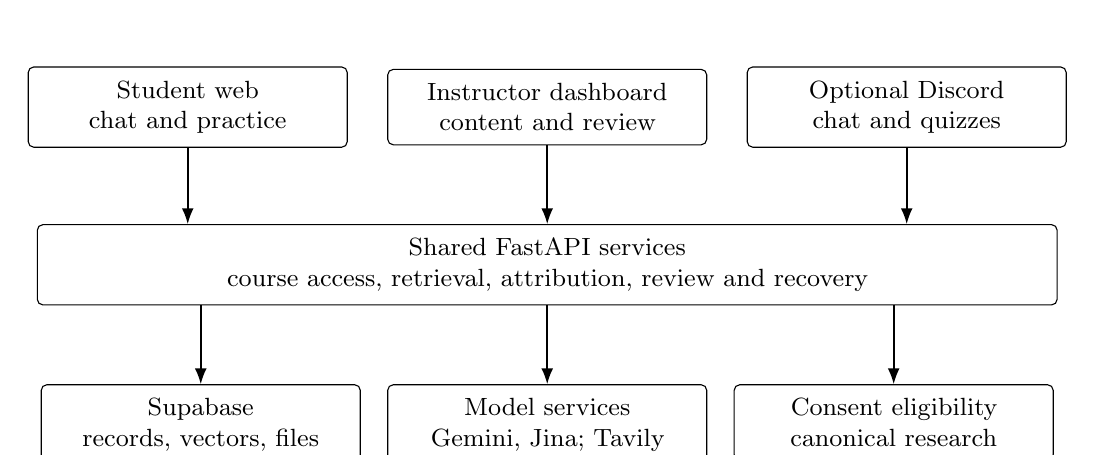
\begin{tikzpicture}[
box/.style={draw,rounded corners=2pt,align=center,font=\small,inner sep=5pt,text width=37mm},
wide/.style={box,text width=126mm},
arr/.style={-{Latex[length=2mm]},semithick}
]
\node[box] (student) {Student web\\chat and practice};
\node[box,right=5mm of student] (staff) {Instructor dashboard\\content and review};
\node[box,right=5mm of staff] (discord) {Optional Discord\\chat and quizzes};
\node[wide,below=10mm of staff] (api) {Shared FastAPI services\\course access, retrieval, attribution, review and recovery};
\node[box,below=10mm of api,xshift=-44mm] (data) {Supabase\\records, vectors, files};
\node[box,below=10mm of api] (provider) {Model services\\Gemini, Jina; Tavily};
\node[box,below=10mm of api,xshift=44mm] (research) {Consent eligibility\\canonical research};
\draw[arr] (student.south) -- (api.north -| student.south);
\draw[arr] (staff.south) -- (api.north);
\draw[arr] (discord.south) -- (api.north -| discord.south);
\draw[arr] (api.south -| data.north) -- (data.north);
\draw[arr] (api.south) -- (provider.north);
\draw[arr] (api.south -| research.north) -- (research.north);
\end{tikzpicture}
\caption{Current component responsibilities. Research capture requires separate consent and study eligibility.}
\label{fig:architecture}
\end{figure}

\section{Preliminary evidence and present limitations}
\subsection{Historical prototype evaluation}
The TALE paper reports 50 cases judged pass/fail by one person for an earlier prototype~\cite{cragpaper}. Table~\ref{tab:historical} separates categories to expose weaker safety performance.

\begin{table}[htbp]
\centering\small
\caption{Reported results for the earlier prototype; not a benchmark of October's system.}
\label{tab:historical}
\begin{tabular}{@{}lrr@{}}
\toprule
Category & Passed/tested & Pass rate\\
\midrule
Grounding & 8/10 & 80\%\\
Fallback & 9/10 & 90\%\\
Robustness & 16/20 & 80\%\\
Safety & 6/10 & 60\%\\
\midrule
Overall & 39/50 & 78\%\\
\bottomrule
\end{tabular}
\end{table}

Reported failures included unnecessary refusals, unsupported out-of-scope answers, ambiguity handling and adversarial or academic-misuse compliance. Small categories, a single judge and unavailable case-level replication materials limit interpretation. These results motivate new tests; they do not validate later corrective retrieval, attribution or access-control changes.

\subsection{CS3103 baseline needs assessment}
The paper reports that 110 eligible CS3103 Computer Networks students were invited and 42 responded and consented, a 38.2\% response rate~\cite{cragpaper}. The local survey export contains 42 responses, comprising 26 Year 3 and 16 Year 4 students. Six closed-response items contain 41 valid answers. Table~\ref{tab:baseline} uses each item's denominator and preserves the distinction between reported habits and observed behaviour.

\begin{table}[htbp]
\centering\small
\caption{Selected baseline findings, cross-checked against local survey aggregates.}
\label{tab:baseline}
\begin{tabularx}{\textwidth}{@{}Yrr@{}}
\toprule
Self-reported habit or desired feature & Count & Percentage\\
\midrule
Uses general AI often or always for study & 35/42 & 83.3\%\\
Usually asks a clarifying follow-up after an unclear answer & 32/41 & 78.0\%\\
Reports at least four prompts per AI conversation & 38/41 & 92.7\%\\
Selects being able to explain the concept as a stopping criterion & 36/41 & 87.8\%\\
Wants instructor-verified answers & 33/41 & 80.5\%\\
Wants citations to exact slide pages & 31/41 & 75.6\%\\
Wants strict grounding in NUS lecture materials & 26/41 & 63.4\%\\
\bottomrule
\end{tabularx}
\end{table}

These findings support prioritising follow-up context, inspectable sources and instructor review. They do not demonstrate that students can correctly evaluate an answer or explain a concept. The prompting categories do not provide an exact mean conversation length. Multiple-selection items may sum above 100\%. The invitation denominator and consent account are taken from the paper; a response CSV alone does not establish the current canonical consent state.

The paper states that access was provided to respondents. Actual uptake, sustained use, attrition and later outcomes remain to be established. The findings describe a self-selected group, so they cannot represent the entire cohort without qualification.

\subsection{What progress establishes}
The present evidence supports a system-development contribution and a motivated evaluation programme. Current source shows extended retrieval, review, practice and research workflows. The historical tests describe earlier behaviour, while the baseline survey describes prior habits and preferences. There is no completed current-system comparison or independent learning-outcome study in this report.

Important remaining risks include stale approved answers or generated questions after material changes, incomplete cross-channel research capture, model-review errors and operational failures spanning storage and database updates. Dashboard mastery and cognitive-category summaries require calibration and careful interpretation. Source-level checks cannot establish deployed access, complete consent operations or real browser and provider behaviour.

\section{Research plan for January--May 2027}
\subsection{Phase 1: Freeze scope and establish a reproducible baseline}
January will establish the study's technical and administrative baseline. The system version, provider models, course corpus, approved-answer state and configuration will be recorded. The priority is to resolve release-blocking ownership, freshness and recovery defects, then exercise representative student, instructor and Discord workflows in staging. This includes permitted and denied accounts, document changes, interrupted submissions and answer updates.

The output will be a versioned system manifest, traceable contribution inventory, failure register and frozen evaluation protocol. The supervisor will review study scope, recruitment feasibility, instruments, data handling and the relevant approval requirements before participant work begins. Sample size and inferential ambitions will depend on realistic recruitment and analysis capacity, not the number of stored messages.

\subsection{Phase 2: Compare technical quality under controlled conditions}
February will evaluate RQ1 using a held-out course-question set reviewed by a subject expert. Coverage should include definitions, mechanisms, comparisons, multi-turn references, insufficient evidence, conflicting evidence and adversarial requests. Development questions and threshold tuning will remain separate from the held-out set.

Three conditions are proposed: single-query RAG, the same pipeline with bounded corrective retrieval, and the full pipeline with answer attribution review. Models, corpus, modes and generation settings will be matched where applicable. Exact approved-answer reuse will be tested in a separate challenge set containing equivalent wording and changed premises; it will not obscure the comparison of generated answers. A general-purpose assistant comparison can be added if budget permits a fair and documented condition.

Independent judges will score correctness, requested-detail coverage, citation support and completeness, and appropriate abstention. Rejections will be reviewed as well as accepted answers. Latency distributions, provider failures, calls and observed token/API costs will be reported. Repeated questions or runs will be analysed as related observations. A frozen result table and error taxonomy will identify whether extra processing produces a worthwhile benefit.

\subsection{Phase 3: Pilot coding and instructor correction}
March will address RQ2 and prepare RQ3. Instructors will review a bounded set of answers using Confirm, Clarify and Dismiss. Measures will include review time, required edits, disagreement, recipient delivery and usefulness of the resulting student update. This will test whether oversight is workable rather than assume that adding a queue reduces staff effort.

A separate coding pilot will establish units of analysis, inclusion rules, examples and category boundaries. At least two coders will independently label a shared sample before adjudication. Agreement and disagreements will be reported using a method appropriate to the final codebook; an ordinal measure is suitable only if the category ordering is justified. Codebook revisions must be followed by a fresh independent reliability sample. Canonical annotation tooling supports this procedure but cannot replace it.

\subsection{Phase 4: Investigate reasoning and revision}
March--April will provisionally host a consented study if approvals, recruitment and the coding pilot permit it. Activities will link an initial explanation or attempted solution, CRAG feedback, evidence inspection and a subsequent explanation of any revision. Structured tasks can elicit observable reasoning, while optional everyday use can show whether similar behaviour occurs without explicit prompting. These conditions will be reported separately.

The primary evidence will be student-produced explanations and revisions, supported by complete interaction context. A pre-task assessment and an independent post-task or delayed transfer/retention task are proposed, subject to course feasibility. Self-reported usefulness and interaction counts will supplement these measures. Participant-level or repeated-measures analysis will account for observations from the same student; message counts will not be treated as independent participants. Unless a suitable comparison design is feasible, findings will remain exploratory associations rather than causal learning claims.

\subsection{Phase 5: Synthesis and final reporting}
April--May will focus on analysis, limitations, final implementation fixes and the final report. The final evidence package will include the system manifest, technical results, error cases, codebook and reliability record, participant flow and approved de-identified analysis outputs. Reports will distinguish invited, consenting, eligible, active and retained participants. Source data will be retained or removed according to the agreed protocol.

\begin{table}[htbp]
\centering\small
\caption{Provisional next-semester milestones and fallback paths.}
\begin{tabularx}{\textwidth}{@{}P{0.16\textwidth}YY@{}}
\toprule
Period & Reviewable deliverable & Fallback if constrained\\
\midrule
January & Baseline manifest; staged workflow checks; approved protocol and instruments & Narrow study scope before recruitment\\
February & Frozen technical comparison; human judgements; latency/cost and failure analysis & Reduce conditions while preserving common questions and independent scoring\\
March & Instructor-workflow pilot; codebook; independent coding reliability results & Revise coding and repeat pilot before longitudinal claims\\
March--April & Eligible interaction dataset; initial reasoning, feedback and revision; independent assessment & Use smaller structured exploratory study; report sparse uptake explicitly\\
April--May & Reproducible analysis; limitations; final report and demonstration & Prioritise technical and methodological contribution if participant evidence is insufficient\\
\bottomrule
\end{tabularx}
\end{table}

\subsection{Risks and success criteria}
Study execution depends on consent and approval, recruitment, course access, instructor availability and reliable capture. Those dependencies will be checked before data collection. Missing context, withdrawal and ineligible records must remain visible in the analysis accounting. Independent outcome tasks and blinded answer review, where feasible, reduce dependence on the same model both producing and judging results.

Technical work will prioritise source revision handling, safe document deletion/recovery, provider deadlines and representative end-to-end checks. Flashcards, notes audits and further adaptive features are secondary to a stable evaluation baseline. If participation is insufficient for longitudinal inference, the project will report technical comparisons and a transparent feasibility study rather than infer development from sparse logs.

Success by May means delivering a reproducible platform and evaluation, an explicit account of where answer correction helps or fails, and appropriately qualified evidence about instructor and student workflows. A positive learning effect is a result to test, not a completion requirement that can be guaranteed in advance.

\section{Conclusion}
The project extends a substantial student-built CRAG foundation towards dependable evidence handling, instructor correction and research-ready interaction records. May--October progress is represented by dated implementation milestones from August onwards, including corrective retrieval, attribution review, controlled answer reuse, contextual practice and consent-aware coding infrastructure. The CS3103 baseline supplies a clear motivation for multi-turn support and instructor-verified sources.

The next stage will evaluate the quality and costs of these design choices and investigate student explanation, critique and revision with independent evidence. This creates a feasible continuation from implemented platform capability to measured technical performance and a defensible educational study.

\clearpage
\begin{thebibliography}{99}
\small
\bibitem{cragpaper}
Ryan Chen Rui Yang, Lim Rik, Ang Zi Jun Dayn, and Bhojan Anand,
``CRAG: An Instructor-Governed Course-Grounded RAG Platform for AI Teaching Assistants in Higher Education,''
IEEE International Conference on Teaching, Assessment and Learning for Engineering (TALE), 2026.
Author-supplied published-paper source, \texttt{main.tex}.
% Author reports publication. Confirm final proceedings metadata, author-name
% formatting, DOI and page numbers against the published record before submission.

\bibitem{repo}
NUS Metaverse Projects, ``getCRAG-ed,'' source repository, inspected 29 October 2026.
Current revision \texttt{35e2a0e}; inherited branch snapshot \texttt{69727bb}.
\url{https://github.com/NUS-Metaverse-Projects/getCRAG-ed}.
% Active evidence: backend/services/query_service.py; retrieval_planner.py;
% note_audit.py; flashcard_service.py; flashcard_scheduler.py;
% onboarding_session_service.py; docs/architecture/10_query_processing.md;
% docs/architecture/11_research_hcd.md; database README; commit history.
% Supplementary private documentation remains outside the submitted source package.

\bibitem{lewis}
P.~Lewis et al., ``Retrieval-Augmented Generation for Knowledge-Intensive NLP Tasks,''
\emph{Advances in Neural Information Processing Systems}, vol.~33, 2020.
\url{https://papers.nips.cc/paper/2020/hash/6b493230205f780e1bc26945df7481e5-Abstract.html}.

\bibitem{yan}
S.-Q.~Yan, J.-C.~Gu, Y.~Zhu, and Z.-H.~Ling,
``Corrective Retrieval Augmented Generation,'' arXiv:2401.15884, 2024.
\url{https://arxiv.org/abs/2401.15884}.

\bibitem{gao}
T.~Gao, H.~Yen, J.~Yu, and D.~Chen,
``Enabling Large Language Models to Generate Text with Citations,''
in \emph{Proceedings of EMNLP}, 2023, pp.~6465--6488.
doi: \href{https://doi.org/10.18653/v1/2023.emnlp-main.398}{10.18653/v1/2023.emnlp-main.398}.

\bibitem{taneja}
K.~Taneja, P.~Maiti, S.~Kakar, P.~Guruprasad, S.~Rao, and A.~K.~Goel,
``Jill Watson: A Virtual Teaching Assistant powered by ChatGPT,''
arXiv:2405.11070, 2024.
\url{https://arxiv.org/abs/2405.11070}.

\bibitem{chi}
M.~T.~H.~Chi, N.~de Leeuw, M.-H.~Chiu, and C.~LaVancher,
``Eliciting Self-Explanations Improves Understanding,''
\emph{Cognitive Science}, vol.~18, no.~3, pp.~439--477, 1994.
\url{https://education.asu.edu/sites/g/files/litvpz656/files/lcl/chideleeuwchiulavancher_3.pdf}.

\bibitem{roediger}
H.~L.~Roediger III and J.~D.~Karpicke,
``Test-Enhanced Learning: Taking Memory Tests Improves Long-Term Retention,''
\emph{Psychological Science}, vol.~17, no.~3, pp.~249--255, 2006.
doi: \href{https://doi.org/10.1111/j.1467-9280.2006.01693.x}{10.1111/j.1467-9280.2006.01693.x}.

\bibitem{hcd}
A.~Bhojan, ``Pedagogical Reflections on the Holistic Cognitive Development (HCD) Framework and AI-Augmented Learning in Creative Computing,''
arXiv:2511.06779, 2025, version~2, January 2026.
\url{https://arxiv.org/abs/2511.06779v2}.
% Uses verified arXiv metadata instead of unconfirmed TALE HCD bibliography entries.

\bibitem{greshake}
K.~Greshake, S.~Abdelnabi, S.~Mishra, C.~Endres, T.~Holz, and M.~Fritz,
``Not what you've signed up for: Compromising Real-World LLM-Integrated Applications with Indirect Prompt Injection,''
arXiv:2302.12173, 2023.
\url{https://arxiv.org/abs/2302.12173}.

\bibitem{ferguson}
R.~Ferguson, ``Ethical Challenges for Learning Analytics,''
\emph{Journal of Learning Analytics}, vol.~6, no.~3, pp.~25--30, 2019.
doi: \href{https://doi.org/10.18608/jla.2019.63.5}{10.18608/jla.2019.63.5}.
\end{thebibliography}

% AUTHOR REVIEW BEFORE SUBMISSION (not rendered)
% 1. Complete title-page fields and confirm official title/module/evaluator.
% 2. Confirm individual ownership of May--October deliverables; add any dated
%    May--July investigation/design records without claiming pre-May contribution.
% 3. Confirm historical pilot dates and original records/rubric where available.
% 4. Complete published TALE bibliographic metadata; acknowledge coauthored work.
% 5. Survey aggregate checks confirm rows/item counts, not live consent eligibility.
% 6. Confirm next-semester calendar, approval pathway, recruitment and instruments.
% 7. Review generated assistance and follow applicable NUS/course disclosure rules.
%    NUS integrity source read: https://www.comp.nus.edu.sg/cug/plagiarism/
% 8. Literature review guidance read:
%    https://advice.writing.utoronto.ca/types-of-writing/literature-review/
% 9. User-provided submission instruction: send softcopy to supervisor and main
%    evaluator by Wednesday Week 12. Exact date/year not established here.
%    No submission, email, publication or Git operation authorised by this draft.
\end{document}
